\subsection{Experiments 5--8: Temporal Forecasting}

Producing business-as-usual projections from historical data is a fundamental task in environmental data analysis. In this study, we design four experiments to evaluate the performance of various forecasting methods across datasets with different characteristics.

% ---- Experiment 5 - GlobalPlasticsProduction

In Experiment 5, we apply forecasting models to the \texttt{GlobalPlasticsProduction} dataset. This dataset contains 59 samples, making it relatively large for time series analysis. This experiment serves as a benchmark for evaluating model performance on larger datasets. Additionally, we tune hyperparameters using both grid search and random search methods and compare their runtime and performance.

\begin{table}[!ht]
	\centering
	\caption{
		\centering Temporal forecasting performance for global plastic production using grid-search tuning for tunable models. The \textsuperscript{*} marker denotes the SVR variant with \(\gamma\) tuning enabled.
	}
	\begin{tabular}{@{}lccccc@{}}
		\toprule
		\textbf{Experiment}                          & \textbf{MAE}                   & \textbf{RMSE}                  & $\mathbf{R^2}$     & \textbf{WAPE}       & \textbf{MAPE}       \\
		\midrule
		Naive Persistence                            & \(5.338 \times 10^7\)          & \(6.031 \times 10^7\)          & -3.615             & 12.70\%             & 12.31\%             \\
		Drift Baseline                               & \(3.344 \times 10^7\)          & \(3.830 \times 10^7\)          & -0.861             & 7.95\%              & 7.69\%              \\
		Exponential Smoothing                        & \(1.792 \times 10^7\)          & \(2.103 \times 10^7\)          & 0.439              & 4.26\%              & 4.10\%              \\
		Ridge Regression                             & \(3.261 \times 10^7\)          & \(3.421 \times 10^7\)          & -0.484             & 7.76\%              & 7.63\%              \\
		Gaussian Process Regression                  & \(3.722 \times 10^7\)          & \(4.086 \times 10^7\)          & -1.118             & 8.85\%              & 8.63\%              \\
		\textbf{Support Vector Regression}           & \(\mathbf{7.921 \times 10^6}\) & \(\mathbf{9.942 \times 10^6}\) & \(\mathbf{0.875}\) & \(\mathbf{1.88}\)\% & \(\mathbf{1.80}\)\% \\
		Support Vector Regression\textsuperscript{*} & \(2.590 \times 10^7\)          & \(2.806 \times 10^7\)          & 0.001              & 6.16\%              & 6.02\%              \\
		Theil-Sen Regression                         & \(1.111 \times 10^7\)          & \(1.365 \times 10^7\)          & 0.764              & 2.64\%              & 2.53\%              \\
		ARIMA Regression                             & \(2.103 \times 10^7\)          & \(2.477 \times 10^7\)          & 0.222              & 5.00\%              & 4.81\%              \\
		\hline
	\end{tabular}
	\label{tab:global_forecasting_grid_search_metrics}
\end{table}

% results/global_forecasting_random_search/metric_table
\begin{table}[!ht]
	\centering
	\caption{\centering Temporal forecasting performance for global plastic production using random-search tuning for tunable models. The \textsuperscript{*} marker denotes the SVR variant with \(\gamma\) tuning enabled.}
	\begin{tabular}{@{}lcccccc@{}}
		\toprule
		\textbf{Experiment}    & \textbf{MAE}                   & \textbf{RMSE}                  & $\mathbf{R^2}$     & \textbf{WAPE}       & \textbf{sMAPE}      \\
		\midrule
		Naive Persistence      & \(5.338 \times 10^7\)          & \(6.031 \times 10^7\)          & -3.615             & 12.70\%             & 13.32\%             \\
		Drift Baseline         & \(3.344 \times 10^7\)          & \(3.830 \times 10^7\)          & -0.861             & 7.95\%              & 8.09\%              \\
		Exponential Smoothing  & \(1.792 \times 10^7\)          & \(2.103 \times 10^7\)          & 0.439              & 4.26\%              & 4.22\%              \\
		Theil--Sen Regression   & \(1.111 \times 10^7\)          & \(1.365 \times 10^7\)          & 0.764              & 2.64\%              & 2.58\%              \\
		ARIMA Regression       & \(1.883 \times 10^7\)          & \(2.225 \times 10^7\)          & 0.372              & 4.48\%              & 4.44\%              \\
		Ridge Regression       & \(2.657 \times 10^7\)          & \(2.834 \times 10^7\)          & -0.019             & 6.32\%              & 6.41\%              \\
		GPR                    & \(3.722 \times 10^7\)          & \(4.086 \times 10^7\)          & -1.118             & 8.85\%              & 9.08\%              \\
		\textbf{SVR}           & \(\mathbf{6.784 \times 10^6}\) & \(\mathbf{8.490 \times 10^6}\) & \(\mathbf{0.909}\) & \(\mathbf{1.61}\)\% & \(\mathbf{1.56}\)\% \\
		SVR\textsuperscript{*} & \(2.503 \times 10^7\)          & \(2.727 \times 10^7\)          & 0.057              & 5.95\%              & 6.01\%              \\
		\hline
	\end{tabular}
	\label{tab:global_forecasting_random_search_metrics}
\end{table}


Table~\ref{tab:global_forecasting_grid_search_metrics} and Table~\ref{tab:global_forecasting_random_search_metrics} indicate that SVR achieved the best overall performance among all evaluated methods. Under the random search tuning setting, SVR attained the lowest MAE, RMSE, WAPE, and MAPE, as well as the highest \(R^2\) value. Under the grid search setting, SVR also remained the top-performing method, although its performance was slightly inferior to that of the random search setting.

\begin{figure}[H]
	\centering
	\subfloat[Theil-Sen regression.]{
		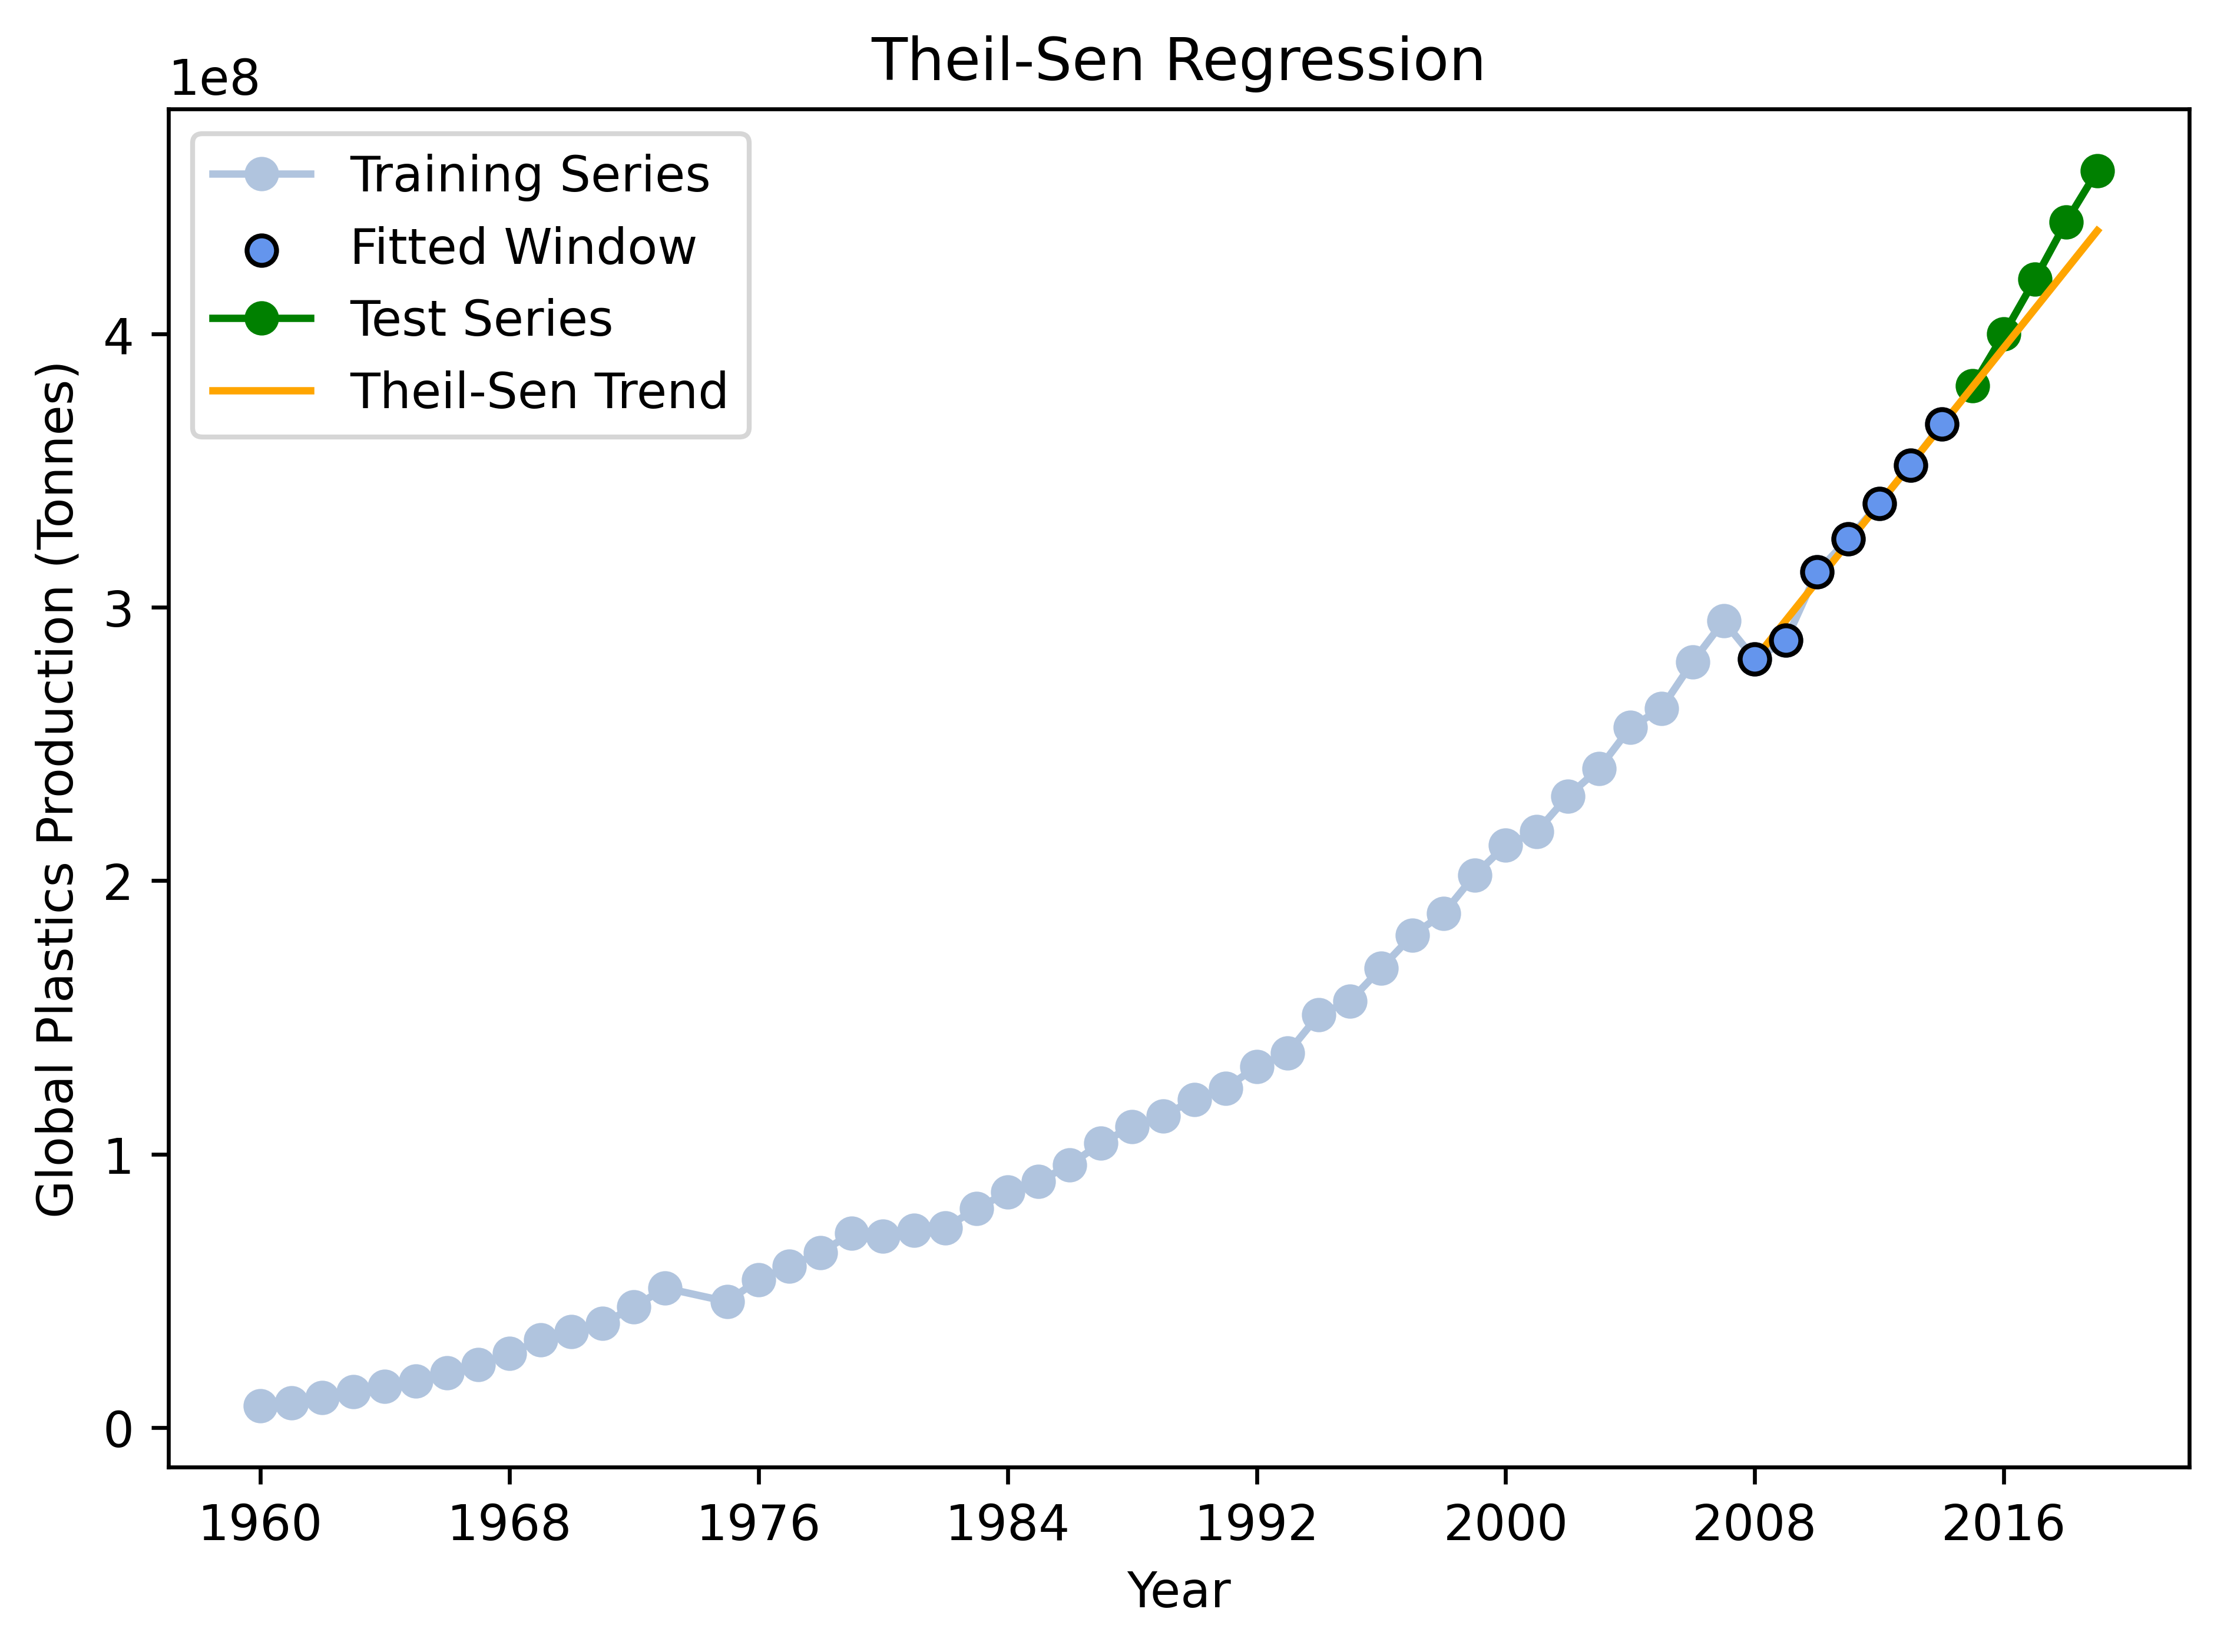
\includegraphics[width=0.45\textwidth]{figures/global_forecasting_theil_sen_regression.png}
	}
	\hfill
	\subfloat[Ridge regression.]{
		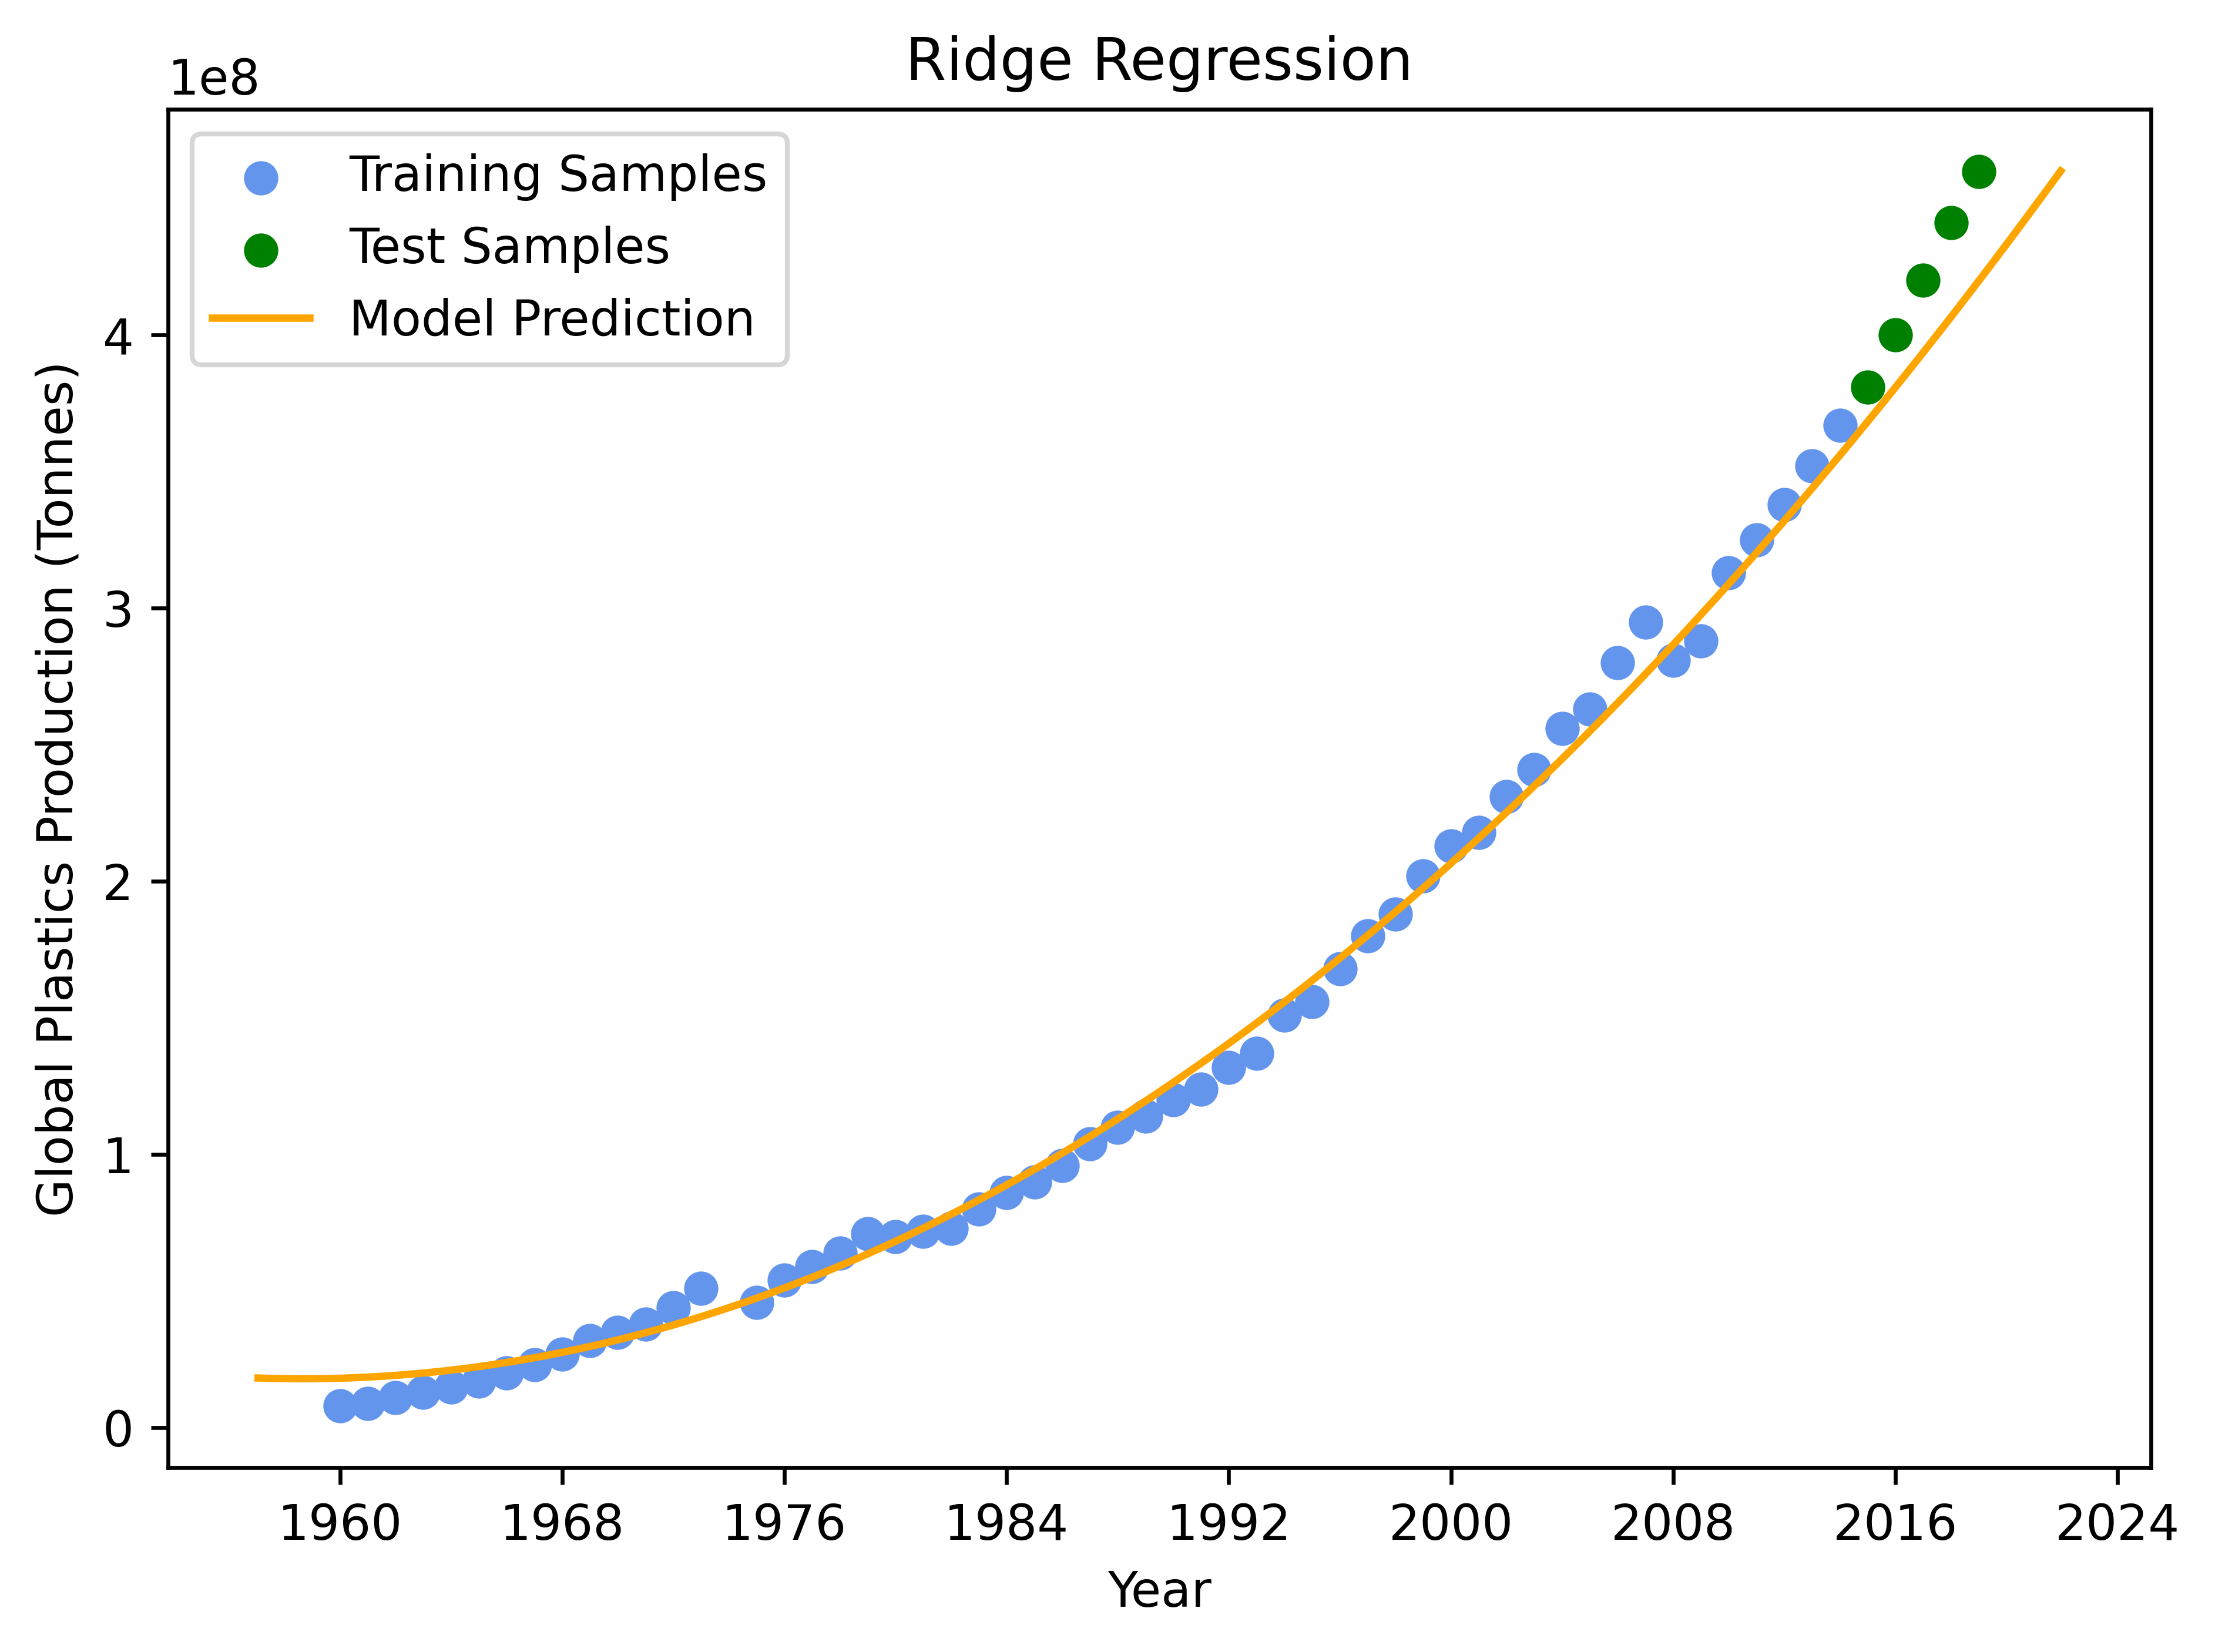
\includegraphics[width=0.45\textwidth]{figures/global_forecasting_ridge_regression.png}
	}

	\vspace{0.5cm}

	\subfloat[GPR.]{
		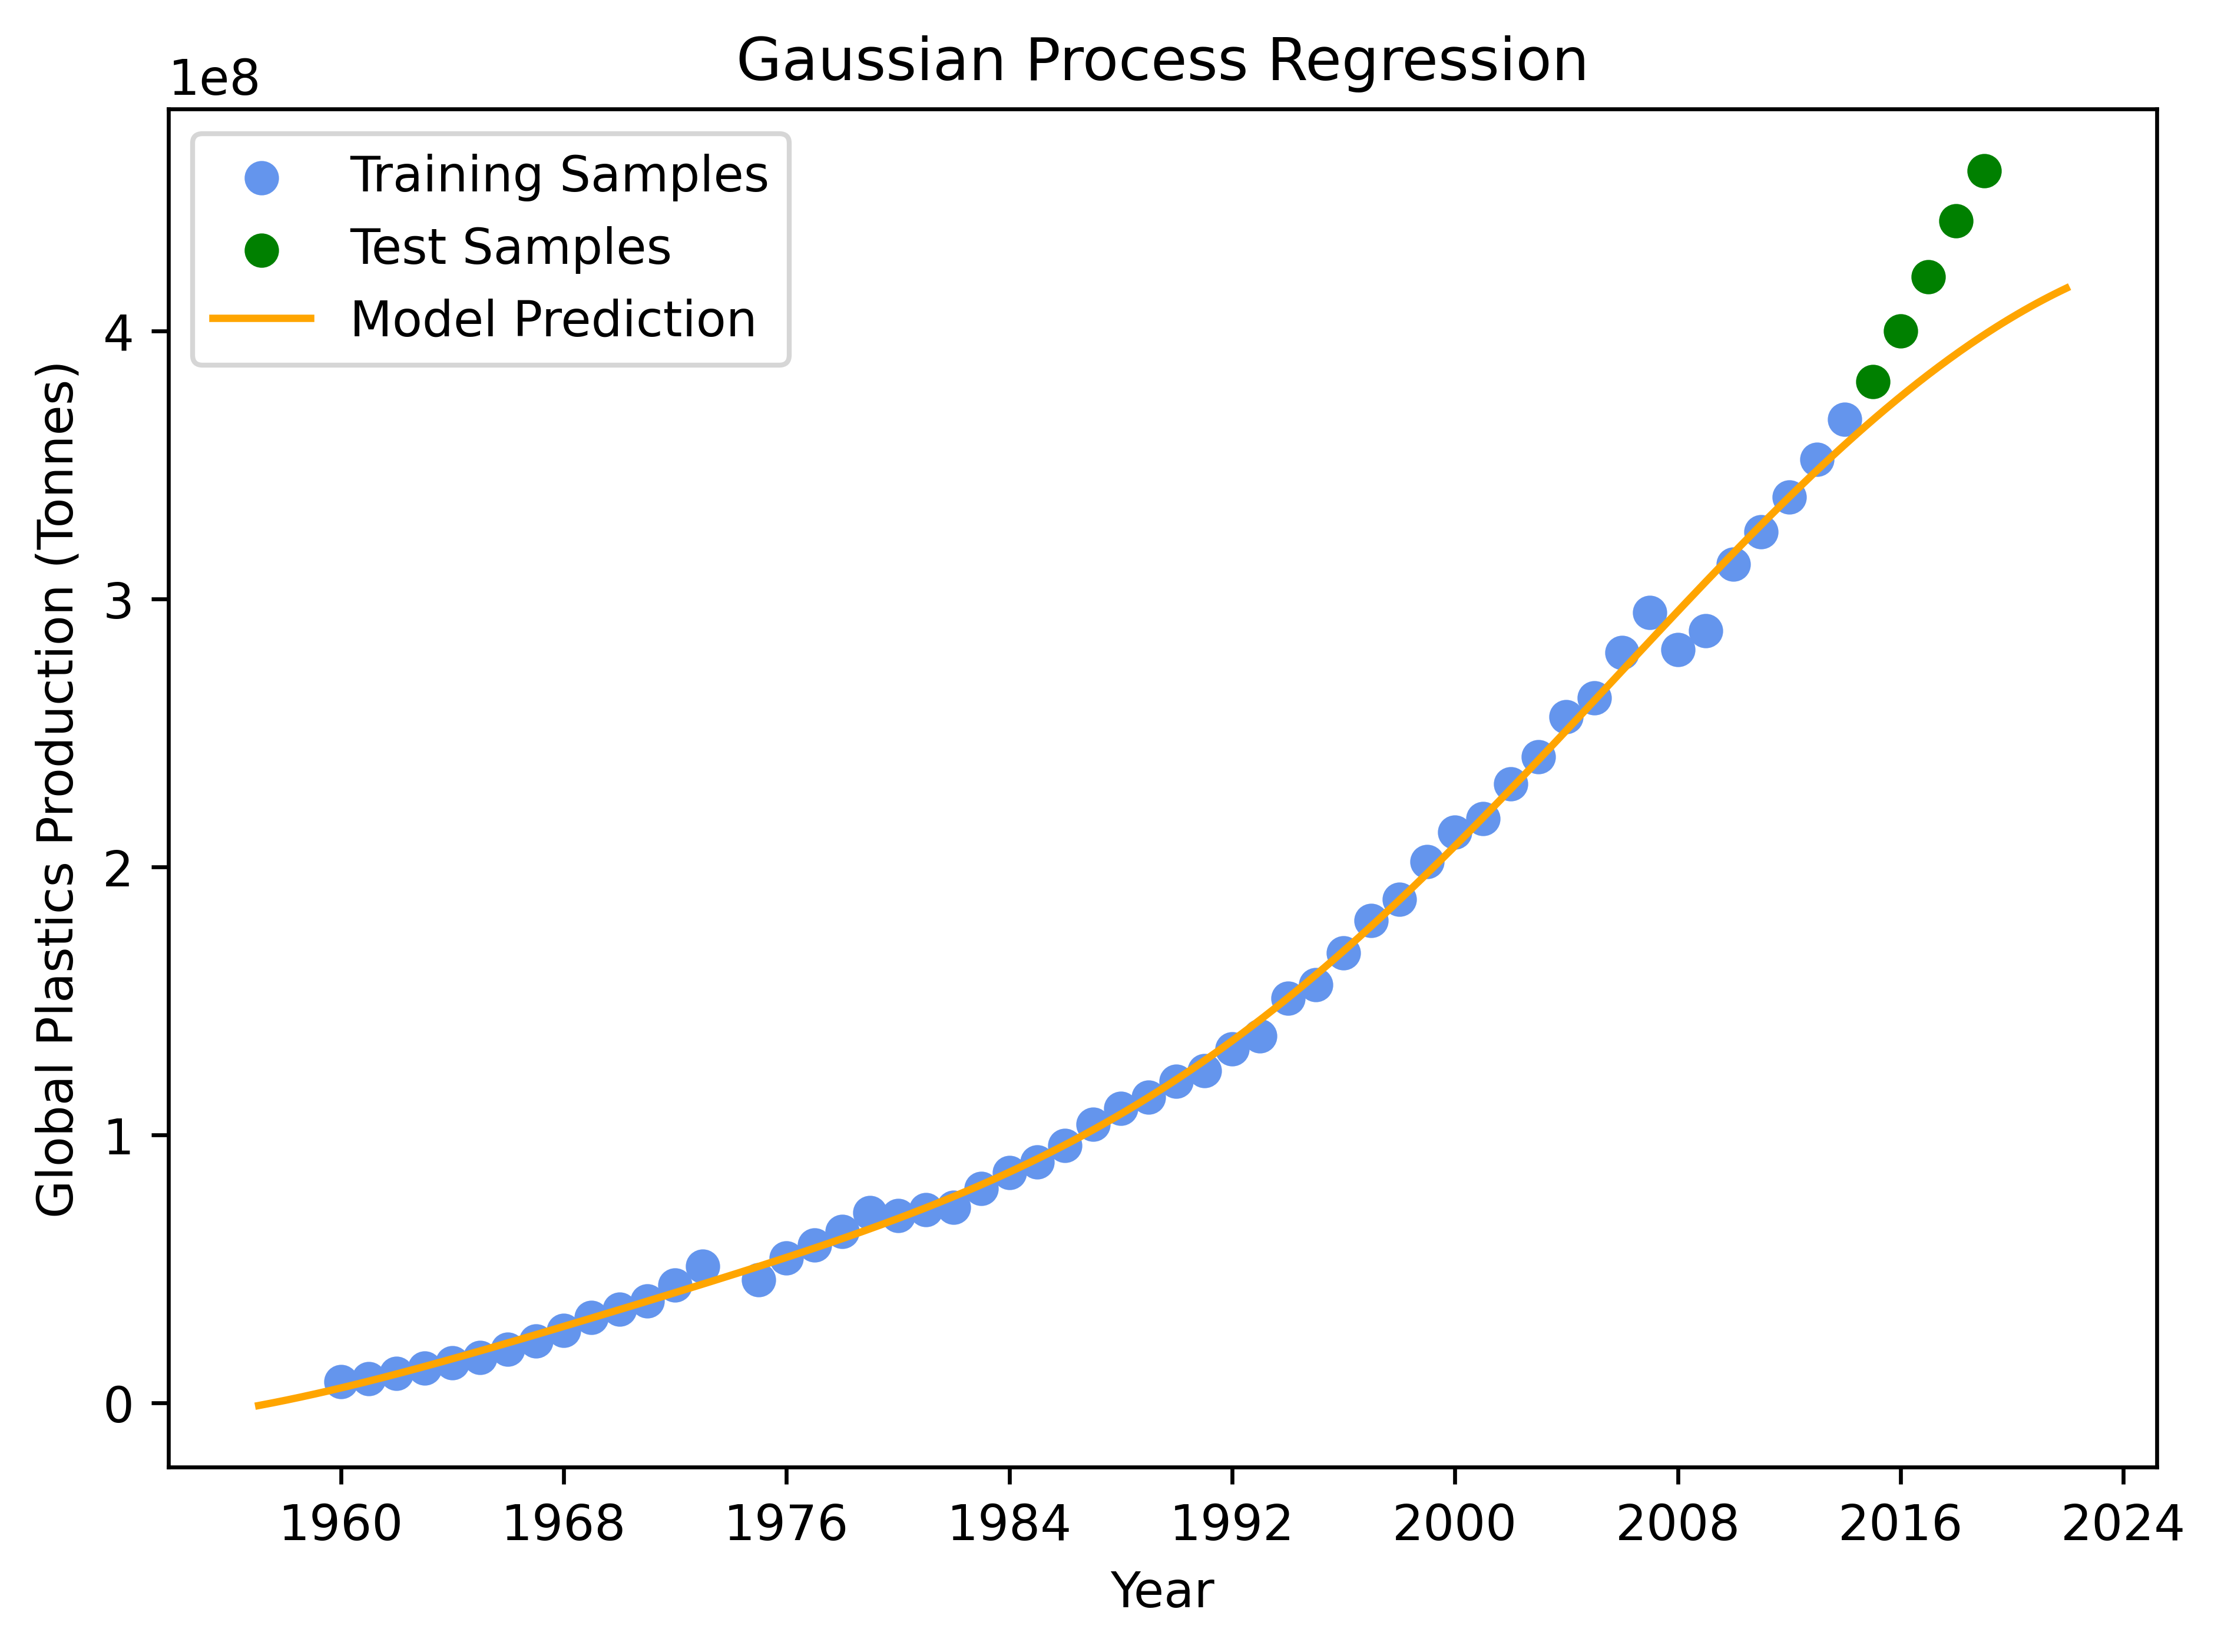
\includegraphics[width=0.45\textwidth]{figures/global_forecasting_gpr.png}
	}
	\subfloat[SVR.]{
		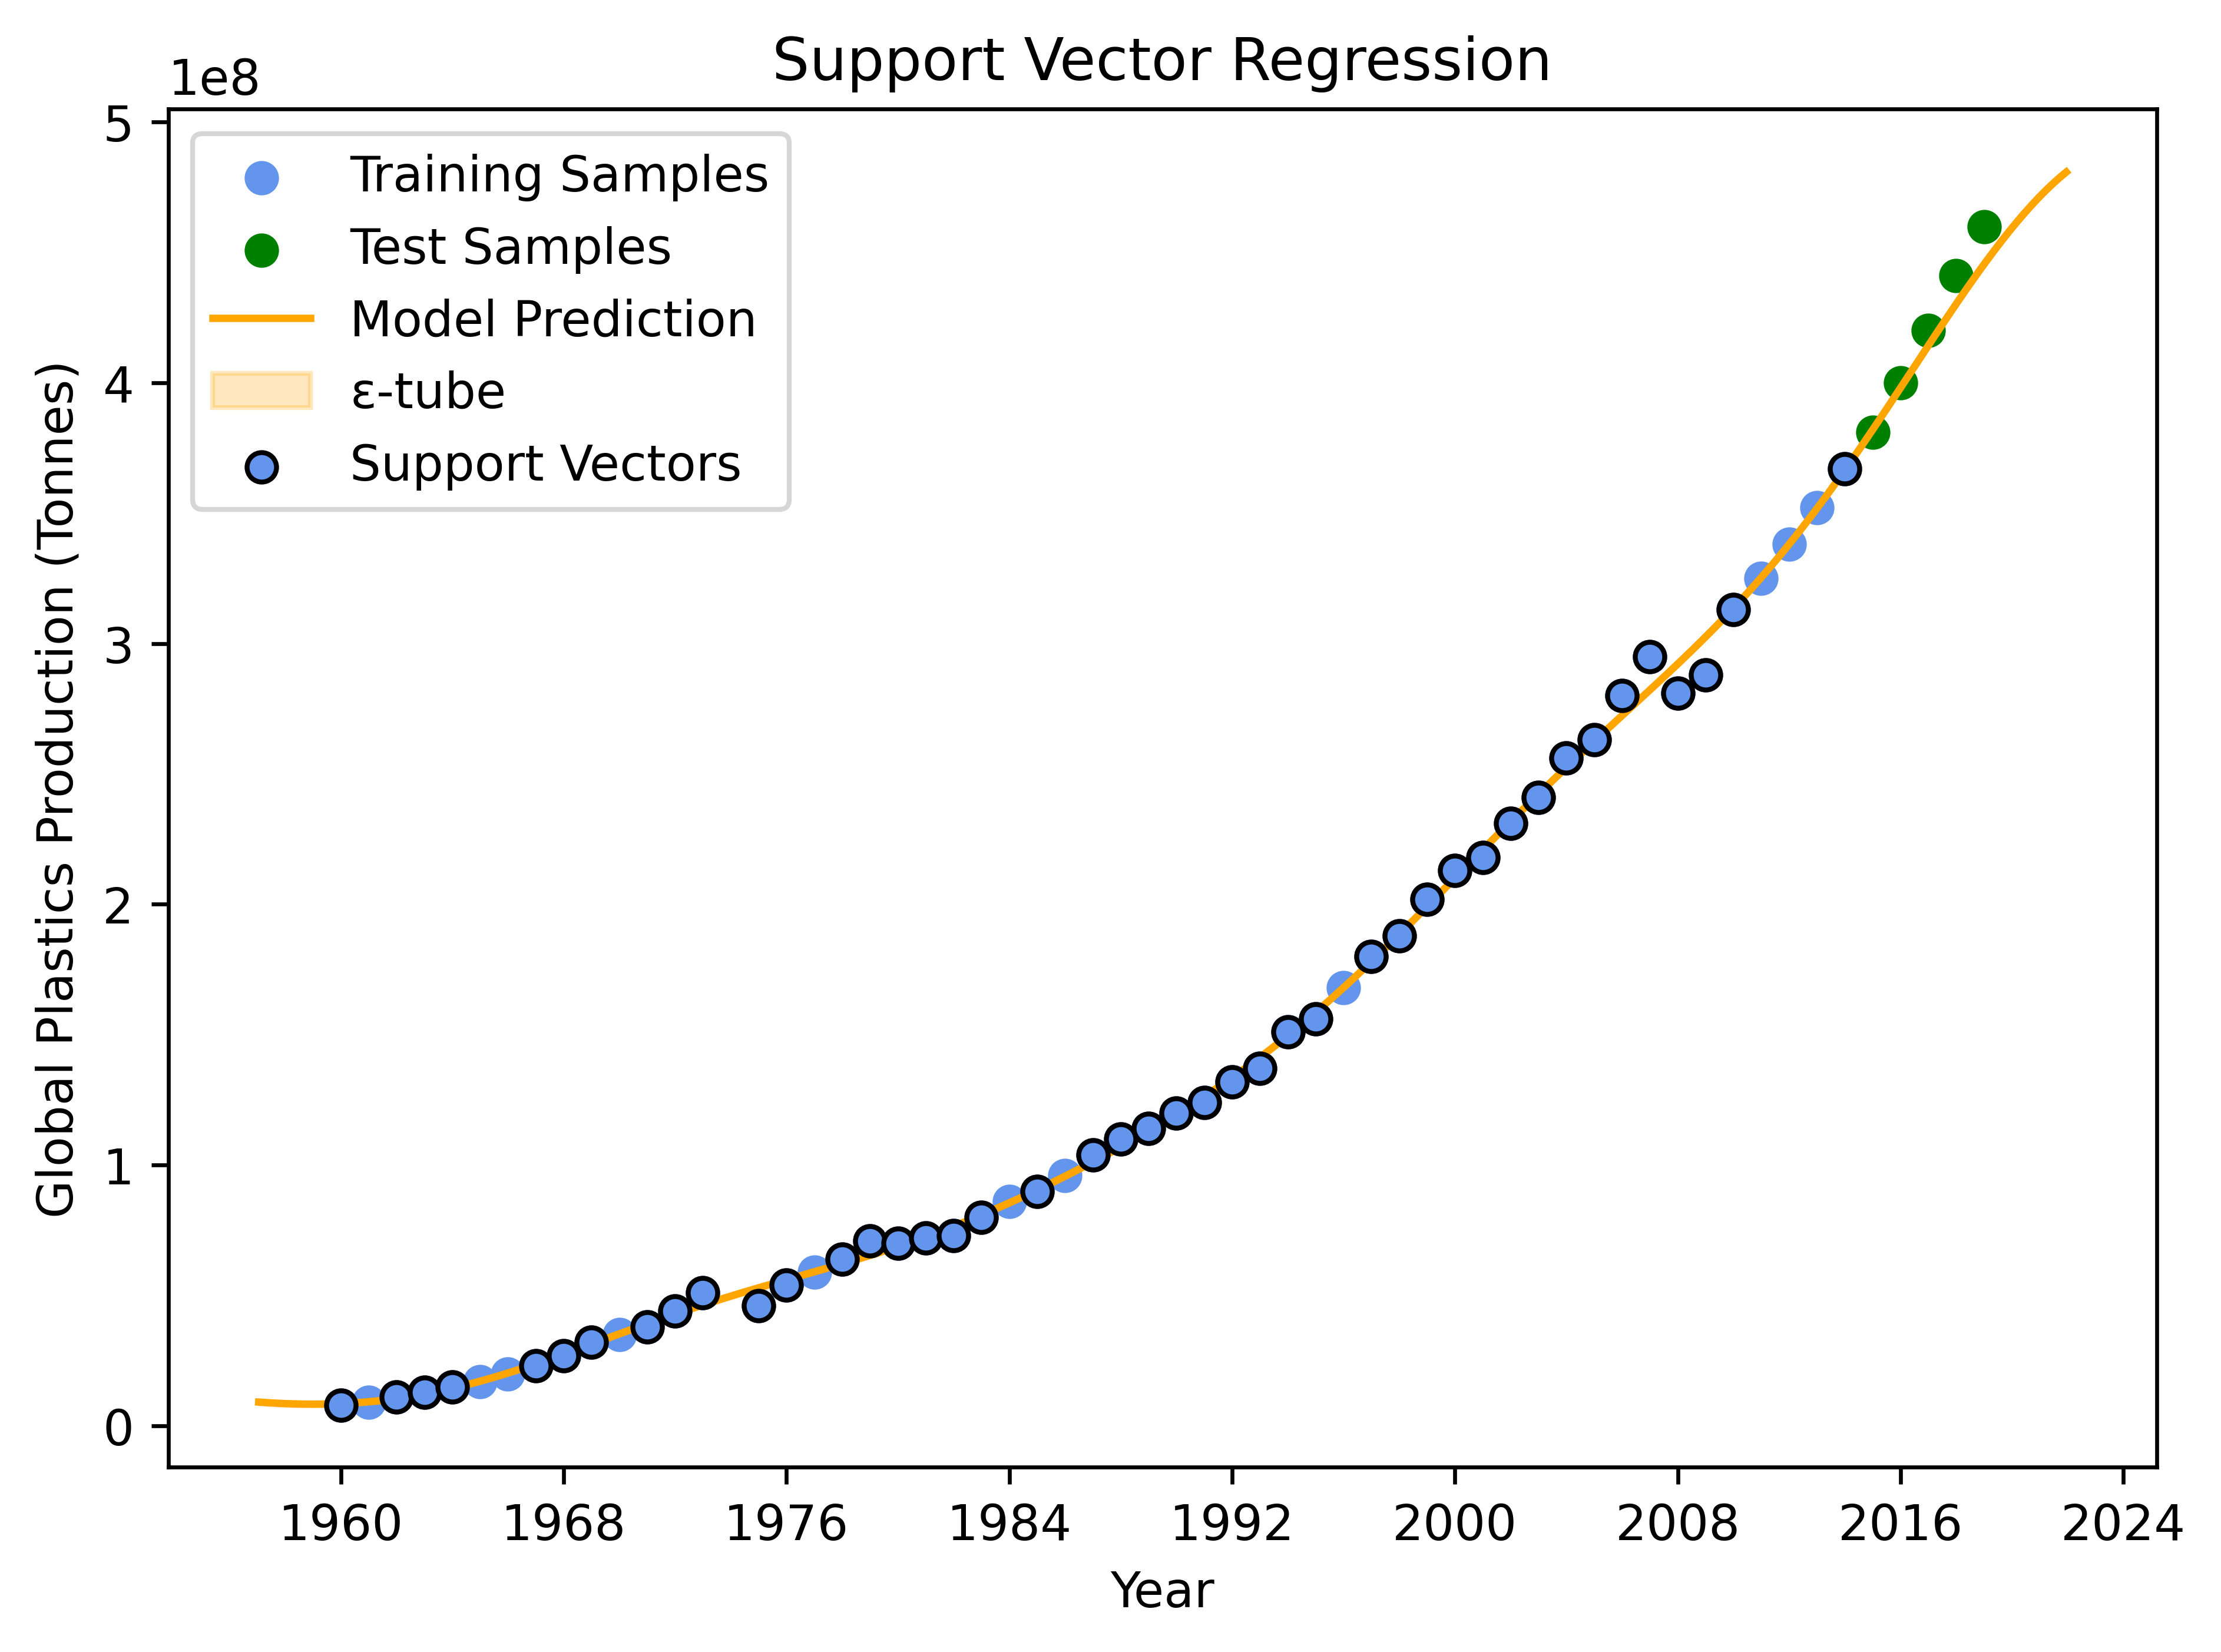
\includegraphics[width=0.45\textwidth]{figures/global_forecasting_svr.png}
	}

	\caption{Forecasts of global plastic production produced by four representative regression models.}
	\label{fig:global_forecasting}
\end{figure}


These results show that SVR is the most effective model for capturing the temporal trend in global plastic production in this experiment. Figure~\ref{fig:global_forecasting} further supports this conclusion, as the SVR forecasts closely follow the actual test values, whereas the other methods exhibit larger deviations.

\begin{table}[!ht]
	\centering
	\caption{
		\centering Hyperparameter tuning time for tunable global plastic production forecasting models under grid search and random search. The \textsuperscript{*} marker denotes the SVR variant with \(\gamma\) tuning enabled.
	}
	\begin{tabular}{@{}lcc@{}}
		\toprule
		\textbf{Experiment}                          & \textbf{Grid Search (ms)} & \textbf{Random Search (ms)} \\
		\midrule
		Ridge Regression                             & 6299.250                  & 3007.902                    \\
		Gaussian Process Regression                  & 25048.184                 & 12571.058                   \\
		Support Vector Regression                    & 5355.496                  & 2711.033                    \\
		Support Vector Regression\textsuperscript{*} & 77496.25                  & 2376.757                    \\
		\hline
	\end{tabular}
	\label{tab:global_forecasting_tuning_time}
\end{table}


Table~\ref{tab:global_forecasting_grid_search_metrics} and Table~\ref{tab:global_forecasting_random_search_metrics} also show that, for all tunable models, random search consistently achieves performance that is equal to or better than that of grid search. Furthermore, Table~\ref{tab:global_forecasting_tuning_time} indicates that random search is more efficient in terms of hyperparameter tuning time under the experimental settings considered. Therefore, in the subsequent experiments, we report only the results obtained using random search for the tunable models.

% ---- Experiment 6 - YearPWG (Japan)

In Experiment 6, we evaluate the same forecasting models on the \texttt{YearPWG (Japan)} dataset. This series contains only 26 annual observations, so the hold-out set is small, and the model rankings should be interpreted cautiously.

\begin{figure}[H]
	\centering
	\subfloat[Auto ARIMA regression.]{
		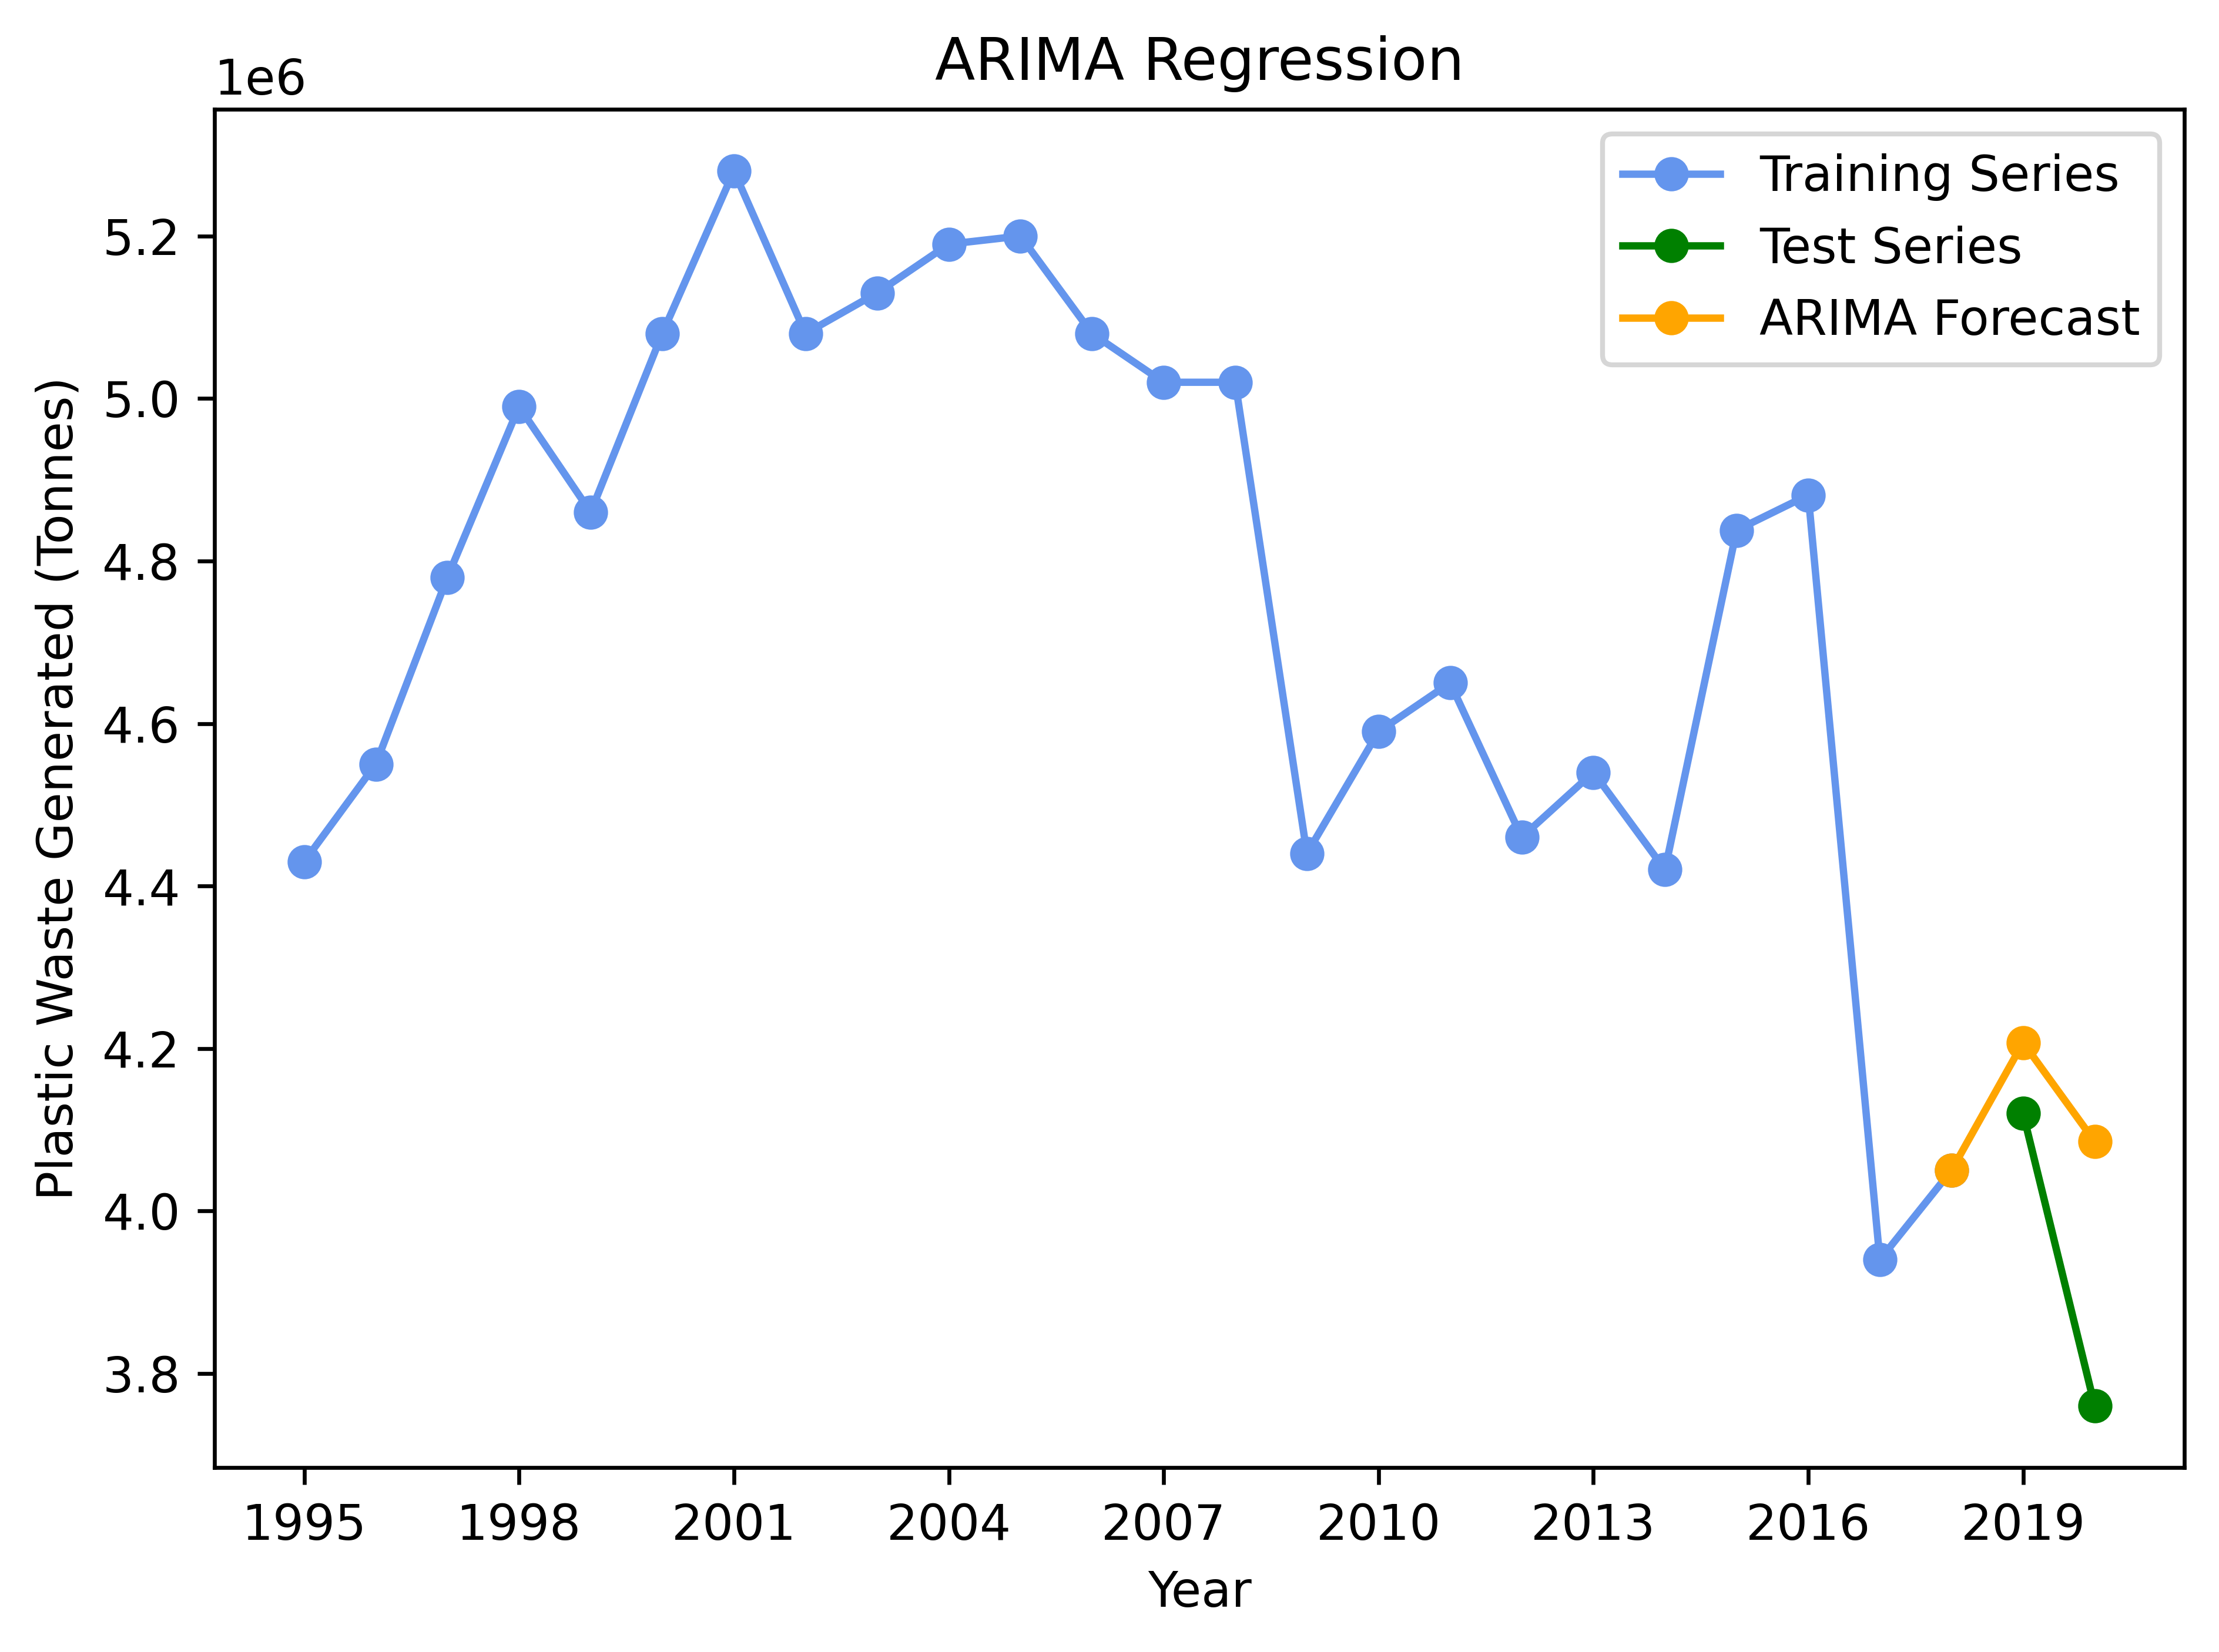
\includegraphics[width=0.45\textwidth]{figures/japan_pwg_forecasting_arima_regression.png}
	}
	\hfill
	\subfloat[Ridge regression.]{
		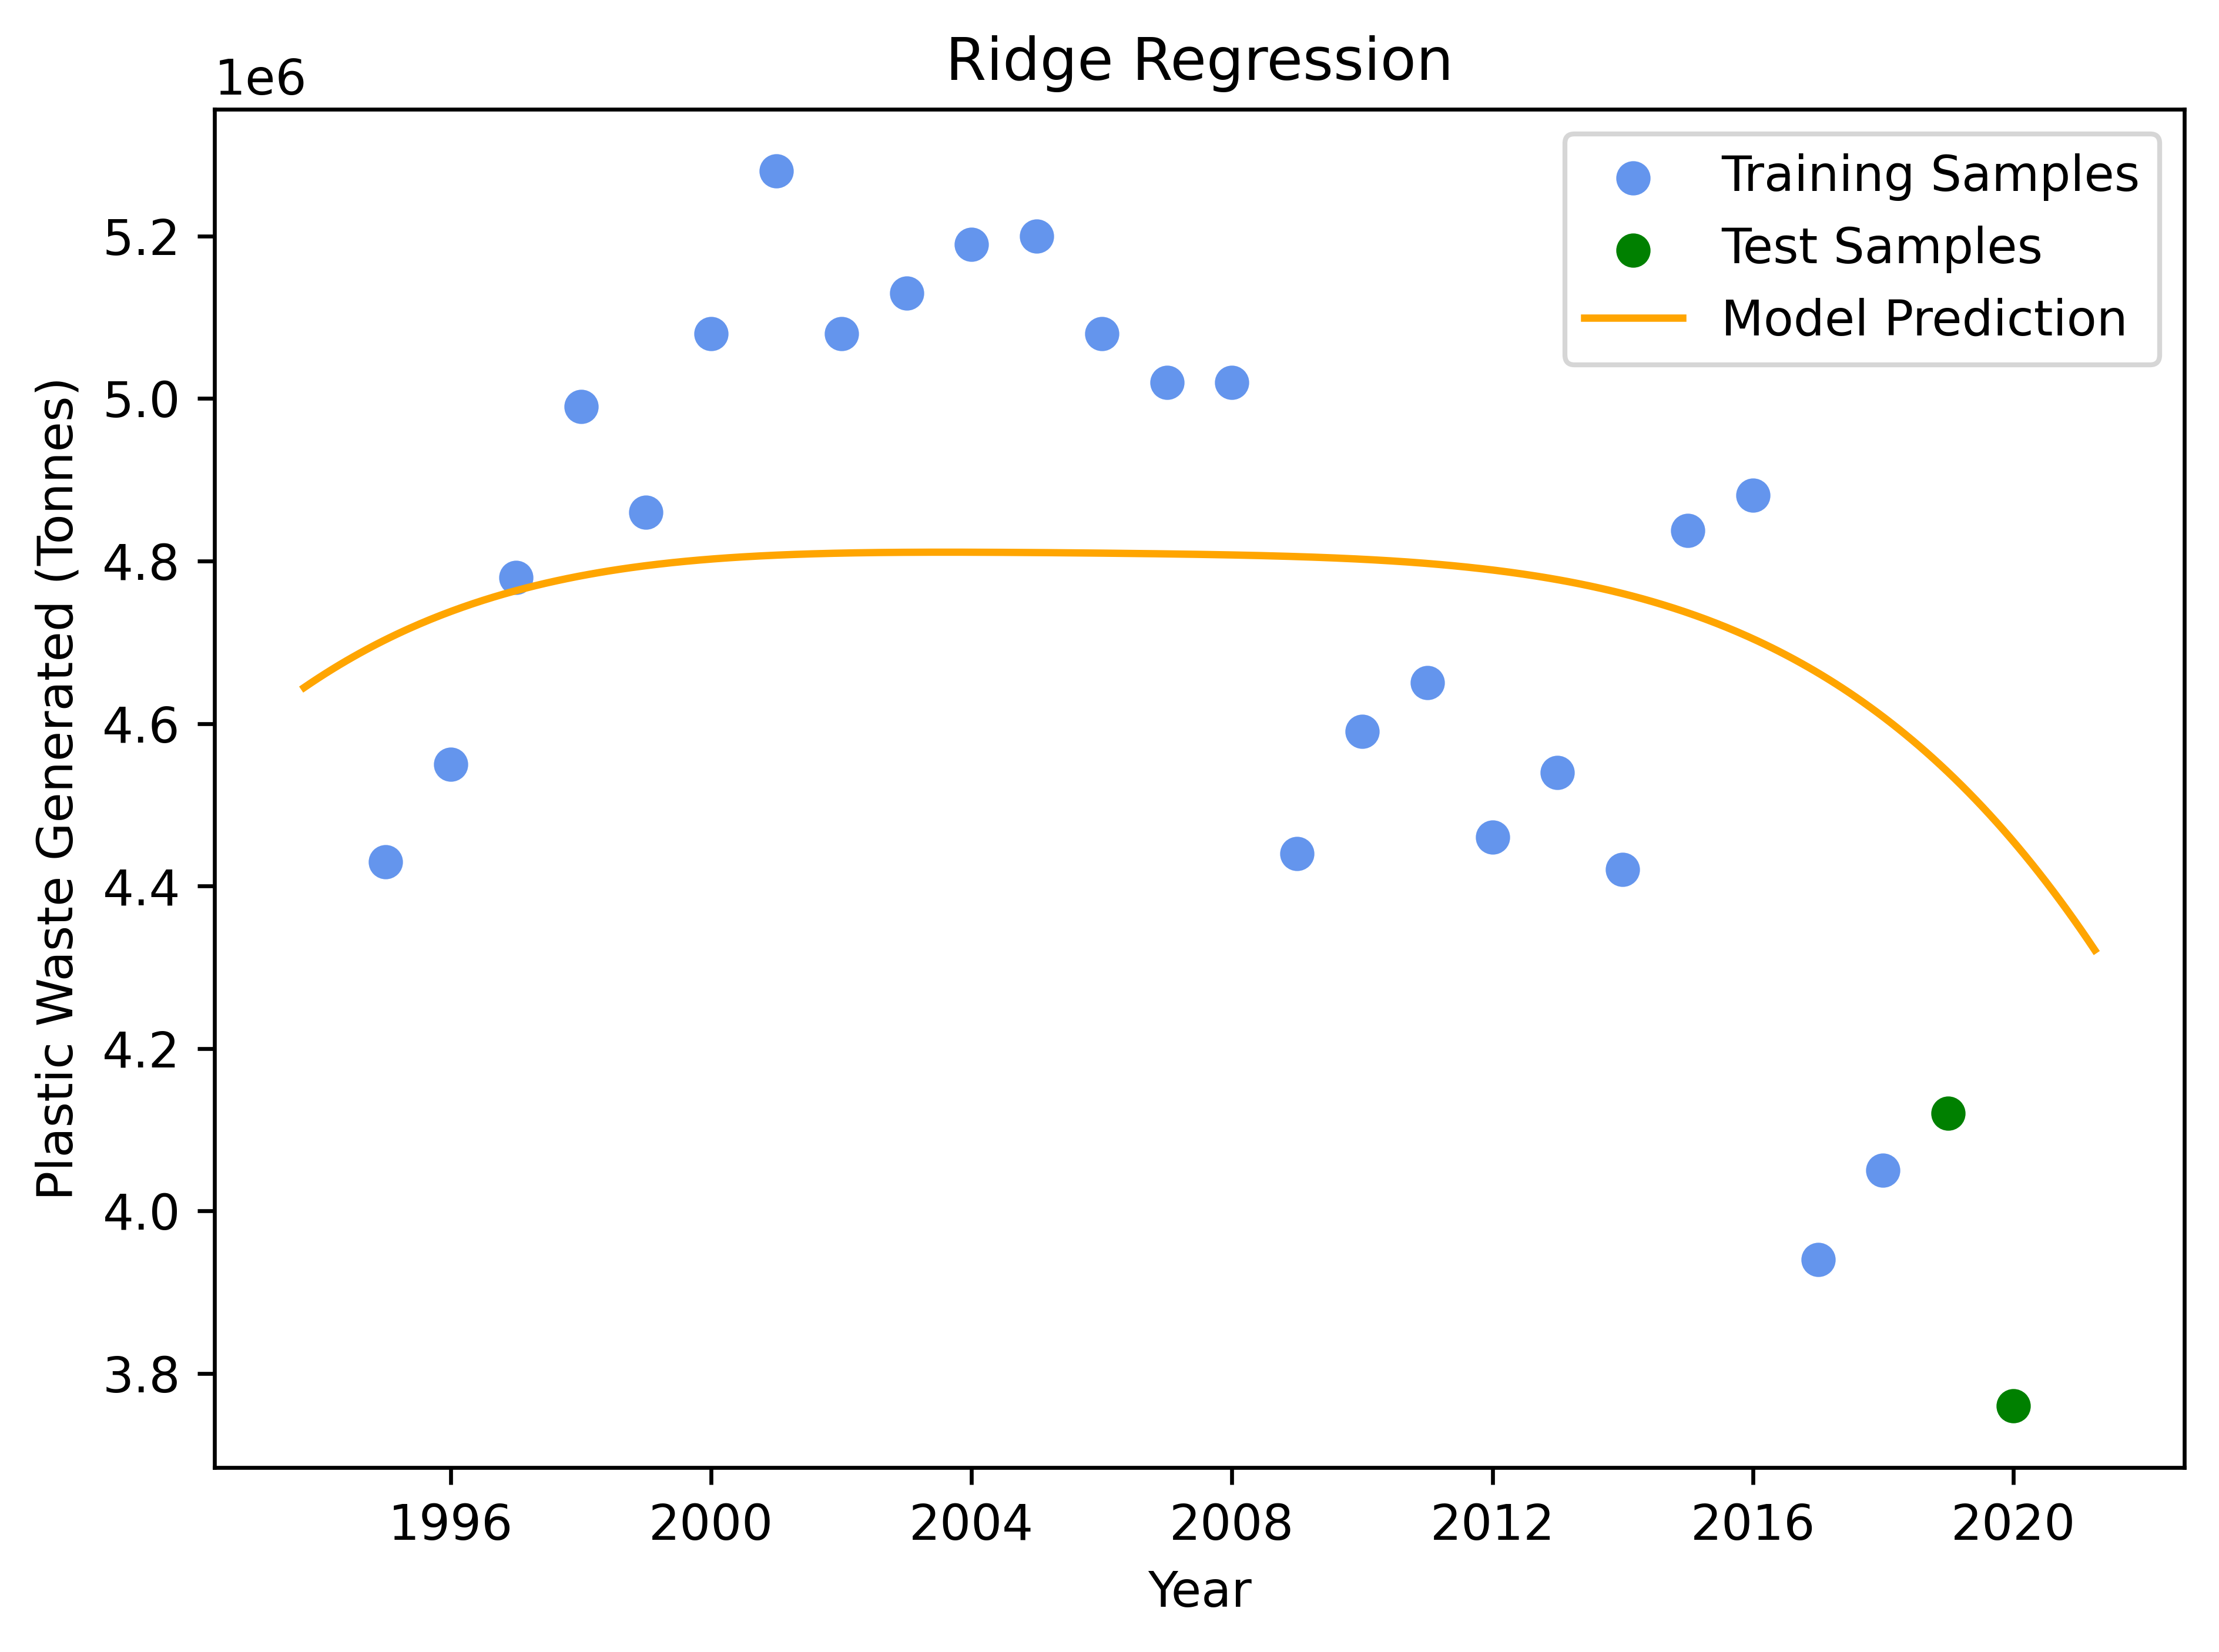
\includegraphics[width=0.45\textwidth]{figures/japan_pwg_forecasting_ridge_regression.png}
	}

	\vspace{0.5cm}

	\subfloat[Gaussian process regression.]{
		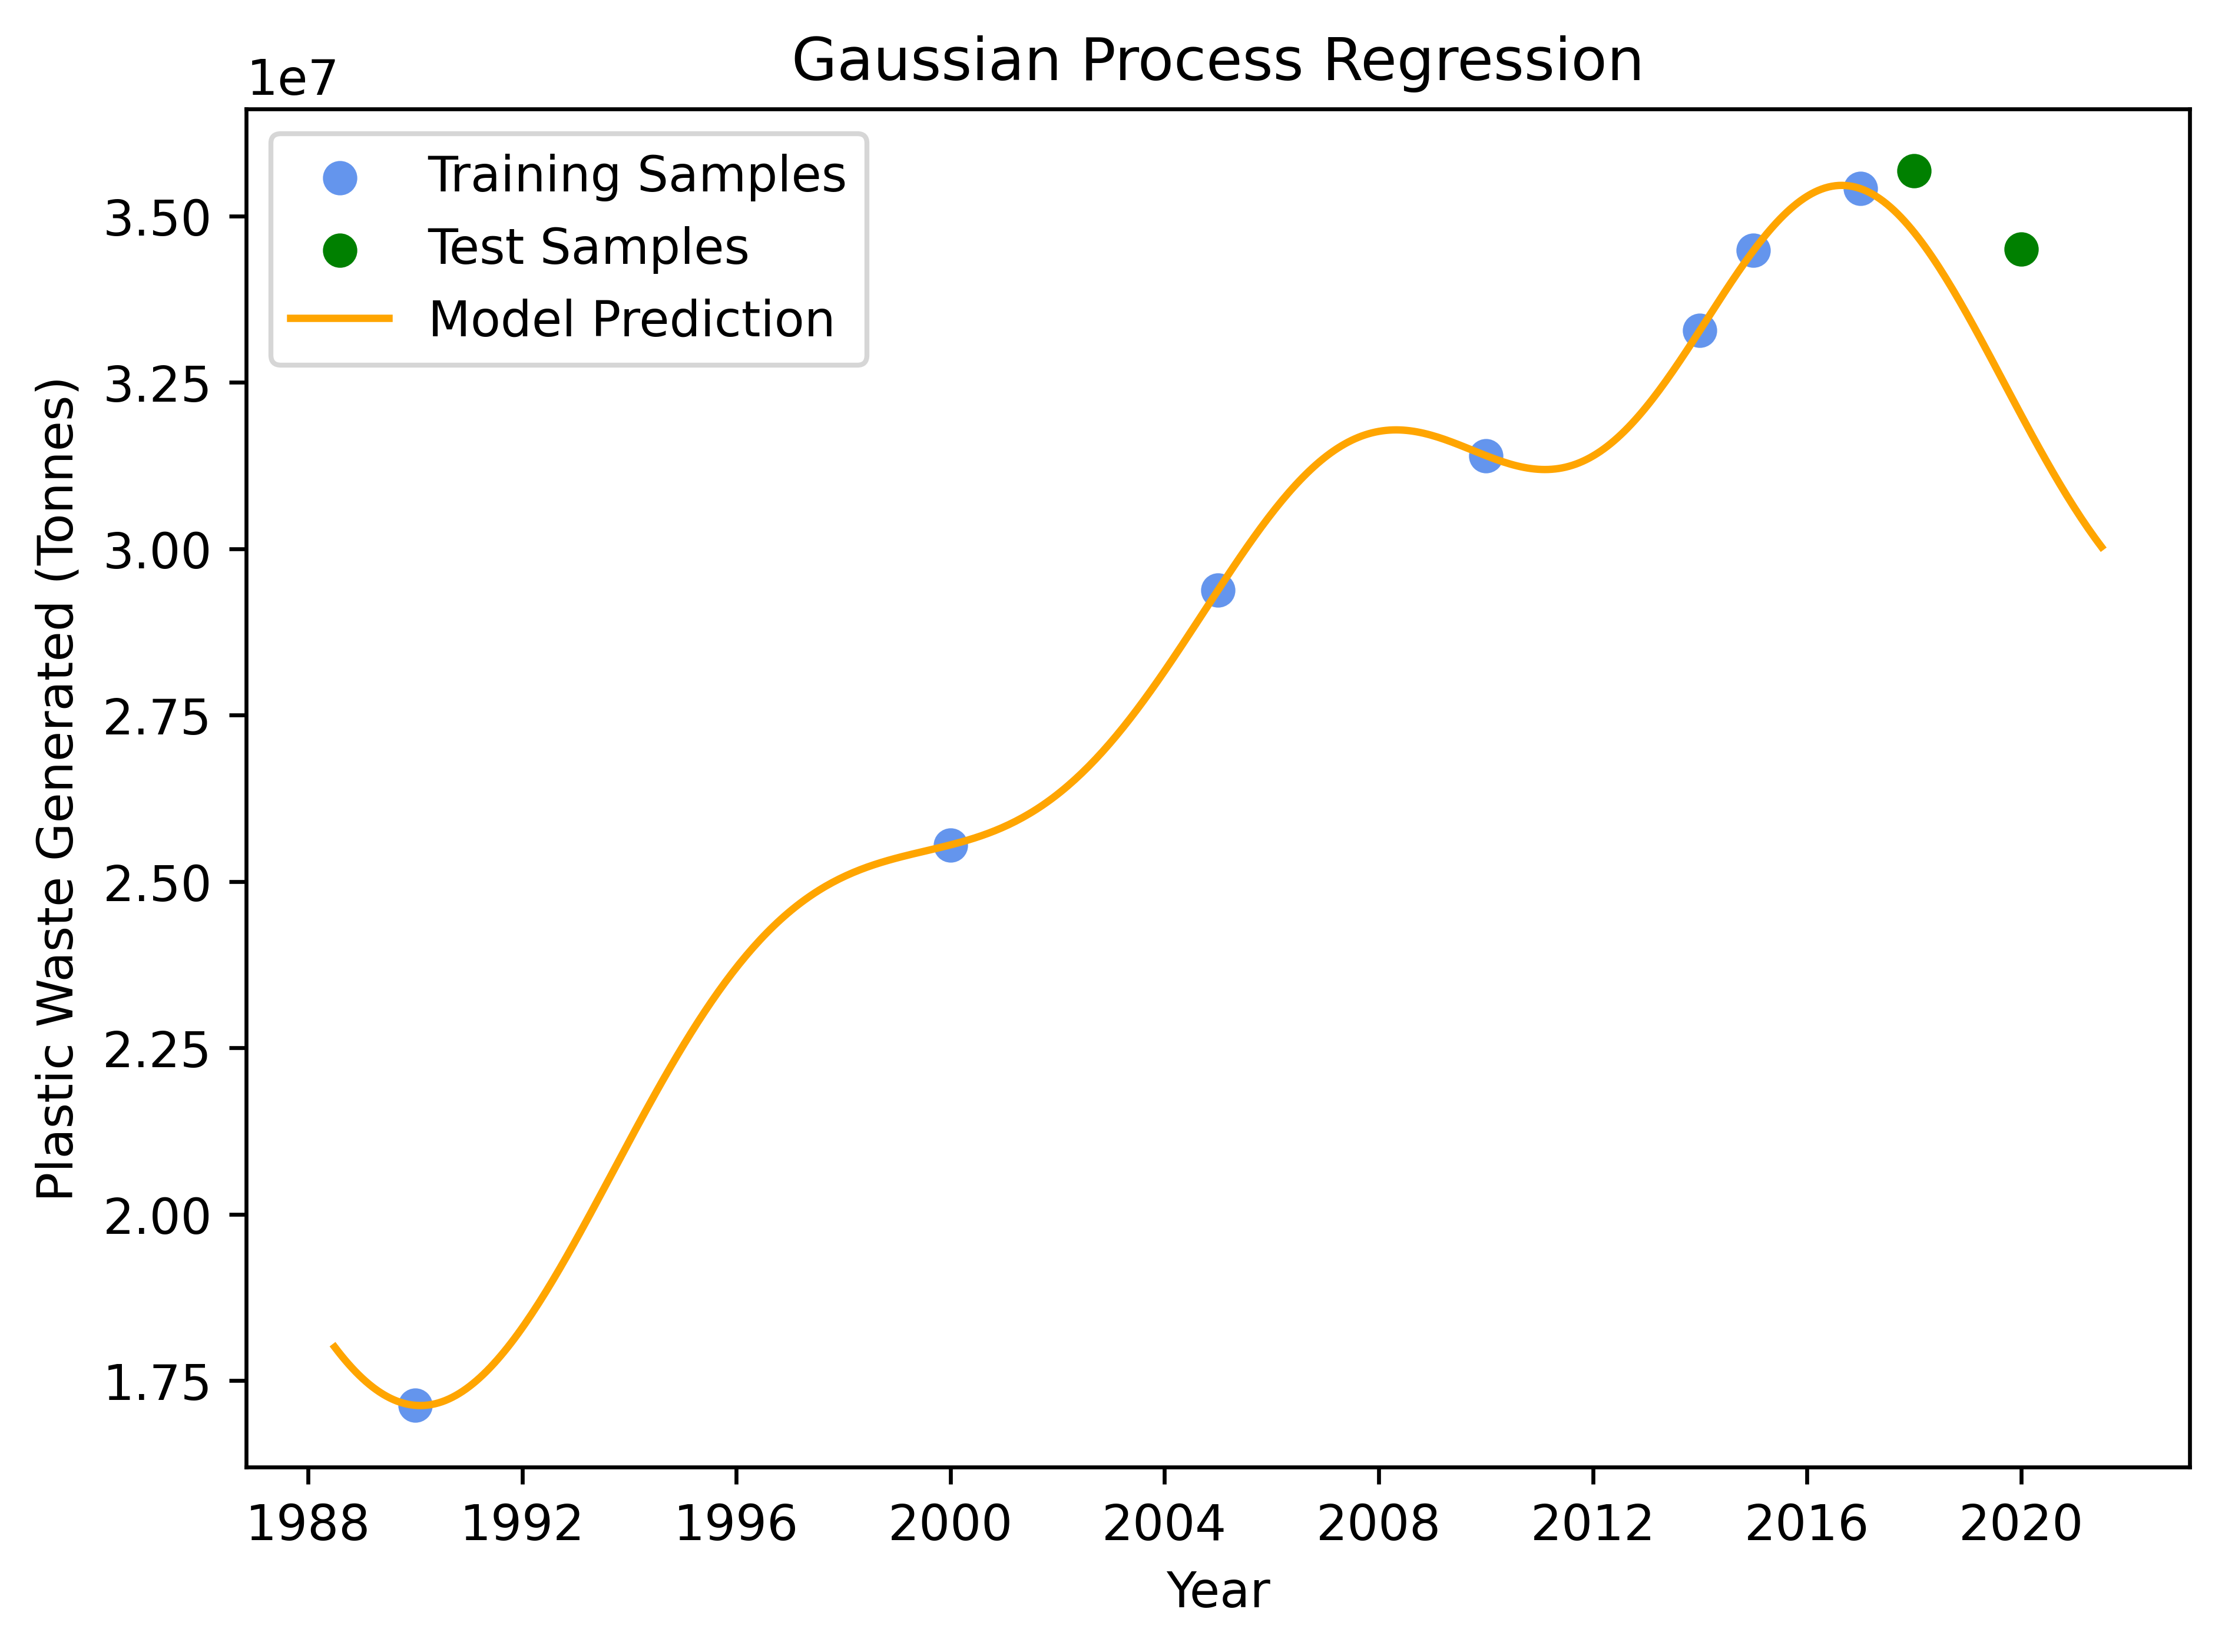
\includegraphics[width=0.45\textwidth]{figures/japan_pwg_forecasting_gpr.png}
	}
	\subfloat[Support vector regression.]{
		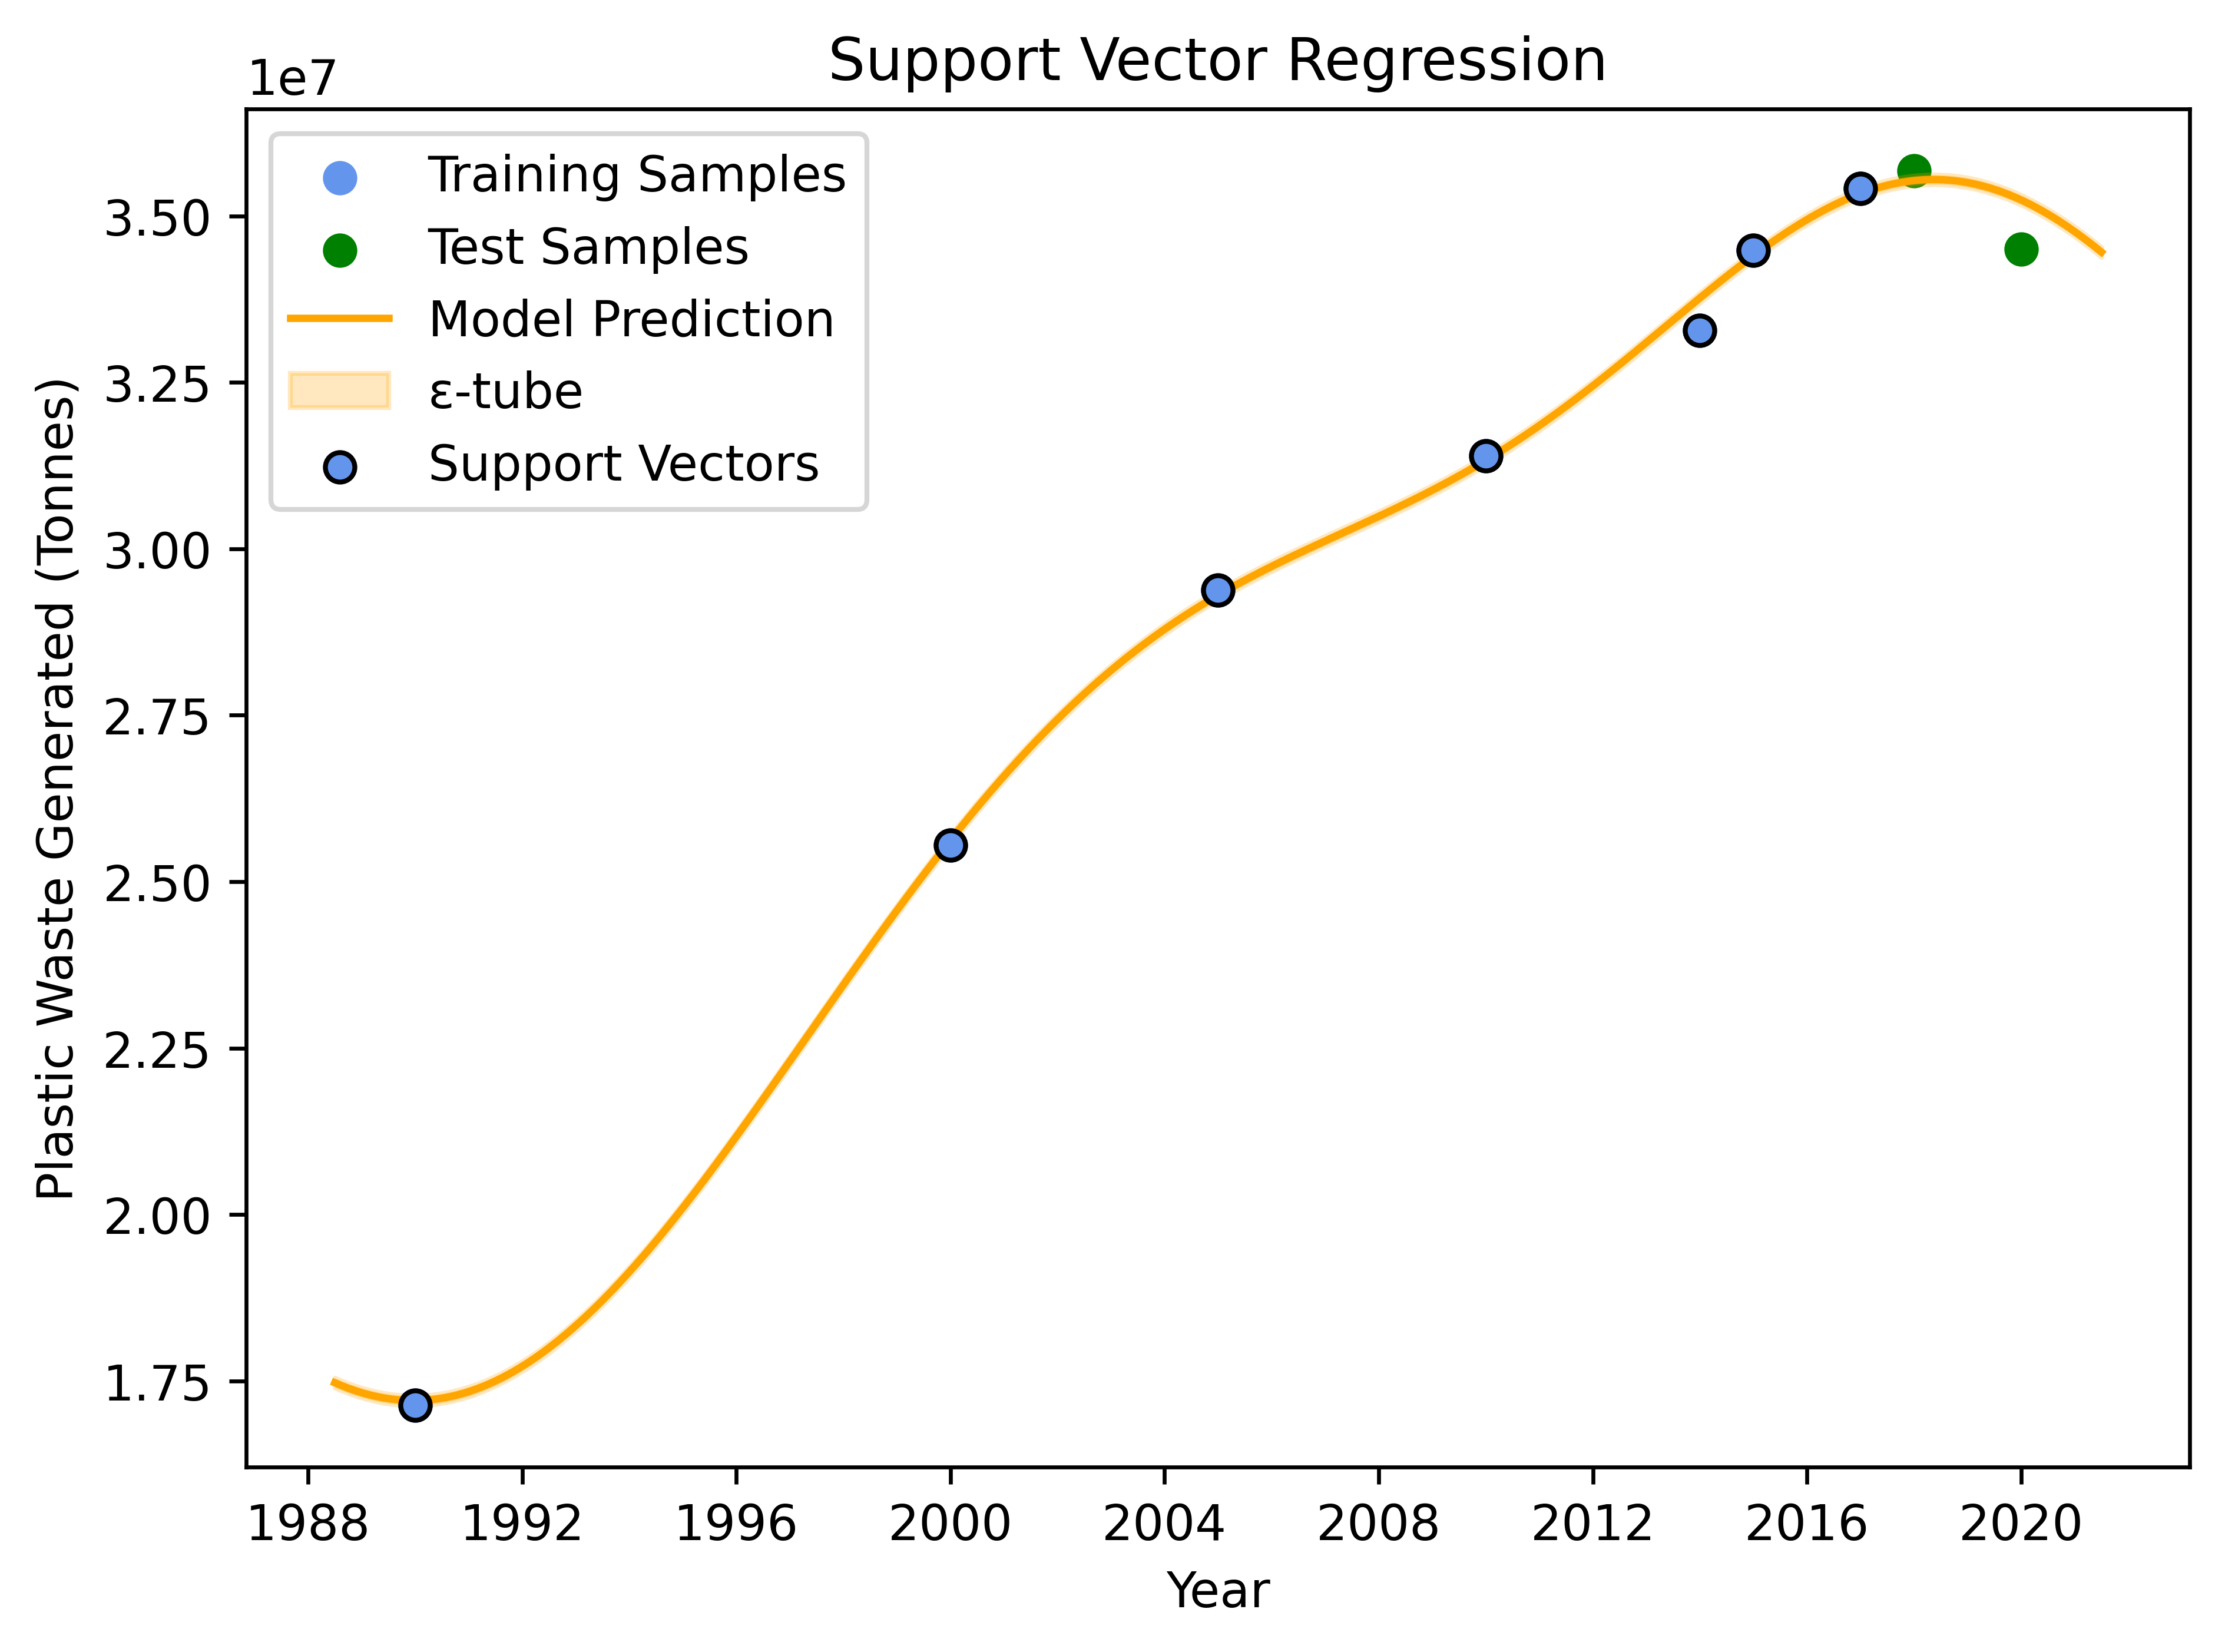
\includegraphics[width=0.45\textwidth]{figures/japan_pwg_forecasting_svr.png}
	}

	\caption{Forecasts of plastic waste generation in Japan by four representative regression models.}
	\label{fig:forecasting_japan_pwg}
\end{figure}

\begin{table}[!ht]
	\centering
	\caption{\centering Temporal forecasting performance for plastic waste generation in Japan using the \texttt{YearPWG (Japan)} dataset.}
	\begin{tabular}{@{}lccccc@{}}
		\toprule
		\textbf{Experiment}                          & \textbf{MAE}                   & \textbf{RMSE}                  & $\mathbf{R^2}$     & \textbf{WAPE}       \\
		\midrule
		Naive Persistence                            & \(5.900 \times 10^5\)          & \(6.712 \times 10^5\)          & -0.294             & 1.68\%              \\
		Drift Baseline                               & \(1.674 \times 10^6\)          & \(2.100 \times 10^6\)          & -11.663            & 4.77\%              \\
		Exponential Smoothing                        & \(2.284 \times 10^6\)          & \(2.742 \times 10^6\)          & -20.591            & 6.51\%              \\
		Theil-Sen Regression                         & \(1.639 \times 10^6\)          & \(2.019 \times 10^6\)          & -10.710            & 4.67\%              \\
		ARIMA Regression                             & \(9.476 \times 10^5\)          & \(1.214 \times 10^6\)          & -3.234             & 2.70\%              \\
		Ridge Regression                             & \(9.447 \times 10^5\)          & \(1.197 \times 10^6\)          & -3.116             & 2.69\%              \\
		GPR                                          & \(1.375 \times 10^6\)          & \(1.742 \times 10^6\)          & -7.715             & 3.92\%              \\
		\textbf{SVR}                                 & \(\mathbf{4.437 \times 10^5}\) & \(\mathbf{5.705 \times 10^5}\) & \(\mathbf{0.065}\) & \(\mathbf{1.26}\)\% \\
		SVR\textsuperscript{*}                       & \(1.430 \times 10^6\)          & \(1.803 \times 10^6\)          & -8.335             & 4.08\%              \\
		\hline
	\end{tabular}
	\label{tab:forecasting_japan_pwg_metrics}
\end{table}


Unlike the global plastics production series, the Japan plastic waste generation series is not monotonic. Figure~\ref{fig:forecasting_japan_pwg} shows that the trend increases in the earlier years, declines sharply, and then partially recovers. This makes the task a useful check of whether flexible regression models can handle short and irregular environmental time series.

Table~\ref{tab:forecasting_japan_pwg_metrics} shows that SVR performs best across all reported metrics, with an MAE of \(4.437 \times 10^5\), an RMSE of \(5.705 \times 10^5\), an \(R^2\) of 0.065, and a WAPE of 1.26\%. The naive persistence baseline is the next-best method by WAPE, while exponential smoothing performs poorly on this short, non-monotonic series.

The differences in model performance between the global plastics production and the Japan plastic waste generation series suggest that model choice depends strongly on both sample size and trend shape. Flexible machine learning models can perform well when the temporal signal is smooth, and enough observations are available, while simple time-series baselines may be more robust for short, non-monotonic country-level series. Combining the data from Experiments 5 and 6, we found that SVR generally performed the best in both experiments.

% ---- Experiment 7: PWDrivers (NN Forecasting)

We speculate that environmental data in this study are influenced by policy factors, but the dataset does not explicitly include policy-related variables. Therefore, we attempt to employ a neural network to capture the implicit relationships between the input features and target variables. In Experiment 7, we apply a multilayer perceptron (MLP) model to the \texttt{PWDrivers} dataset after removing outliers using an isolation forest with a contamination rate \(r_c\). Because we are unsure about the appropriate level of outlier removal, we experiment with a range of contamination rates \(r_c \in \{0.1, 0.2, 0.3, 0.4, 0.45, 0.5\}\). This experiment aims to find out whether the MLP can effectively learn these latent relationships and produce accurate forecasts.

\begin{table}[!ht]
	\centering
	\caption{\centering Neural-network forecasting performance for plastic waste generation on the \texttt{PWDrivers} dataset.}
	\begin{tabular}{@{}lccccc@{}}
		\toprule
		\textbf{Experiment} & \textbf{MAE}             & \textbf{RMSE}         & $\mathbf{R^2}$ & \textbf{WAPE} & \textbf{MAPE} \\
		\midrule
		NN Forecasting      & \(9.146 \times 10^4\)    & \(1.495 \times 10^5\) & 0.726          & 41.22\%       & 92.91\%       \\
		\hline
	\end{tabular}
	\label{tab:nn_forecasting_metrics}
\end{table}


Table~\ref{tab:nn_forecasting_metrics} shows that the MLP is sensitive to the isolation forest contamination rate. When \(r_c \in \{0.1, 0.2\}\), only a small portion of data points is removed, and the performance is poor, with MAPE achieving over 600\% and WAPE over 80\%. The best \(R^2\) value, 0.806, and the lowest WAPE, 37.47\%, occur at \(r_c = 0.3\), suggesting that moderate outlier removal helps the neural network learn the broad relationship between the driver variables and plastic waste generation. The lowest MAE, RMSE, and MAPE occur at \(r_c = 0.45\), with an MAE of \(9.146 \times 10^4\), an RMSE of \(1.495 \times 10^5\), and a MAPE of 92.91\%. When \(r_c\) is increased to 0.5, the performance begins to degrade again, indicating that removing too many observations may discard useful observations.

The lowest WAPE of 37.47\% suggests that the MLP struggles to capture the temporal trend in the pooled \texttt{PWDrivers} dataset with high accuracy, probably due to the heterogeneity of the observations. Hence, this experiment should be treated as an exploratory benchmark for driver-based neural-network forecasting rather than a definitive forecasting model.

% ---- Experiment 8: PWDrivers (Japan & Slovenia); Multivariate Forecasting

In Experiment 8, we conduct multivariate forecasting using GPR, SVR, and MLP models on the \texttt{PWDrivers (Japan)} and \texttt{PWDrivers (Slovenia)} datasets. For the MLP, we first filter the pretraining dataset with an isolation forest using a contamination rate of 0.3, which achieves the lowest WAPE in Experiment 7. Then, we pretrain the model on the \texttt{PWDrivers} dataset excluding data points associated with the target country, and subsequently train it on the target country's training data. This experiment compares the performance of traditional machine learning methods on tiny datasets. For the \texttt{PWDrivers (Slovenia)} dataset, which contains only \(6\) samples, hyperparameter tuning is not performed due to the limited data availability.

\begin{table}[!ht]
	\centering
	\caption{\centering Multivariate forecasting performance for plastic waste generation in Japan using the \texttt{PWDrivers (Japan)} dataset.}
	\begin{tabular}{@{}lccccc@{}}
		\toprule
		\textbf{Experiment}         & \textbf{MAE}                   & \textbf{RMSE}                  & \textbf{WAPE}       \\
		\midrule
		GPR                         & \(4.549 \times 10^5\)          & \(4.562 \times 10^5\)          & 11.14\%             \\
		SVR                         & \(4.782 \times 10^5\)          & \(4.792 \times 10^5\)          & 11.71\%             \\
		\textbf{NN Forecasting}     & \(\mathbf{3.943 \times 10^5}\) & \(\mathbf{3.957 \times 10^5}\) & \(\mathbf{9.65}\)\% \\
		\hline
	\end{tabular}
	\label{tab:multivariate_forecasting_japan_metrics}
\end{table}

\begin{table}[!ht]
	\centering
	\caption{\centering Multivariate forecasting performance for plastic waste generation in Slovenia using the \texttt{PWDrivers (Slovenia)} dataset.}
	\begin{tabular}{@{}lccccc@{}}
		\toprule
		\textbf{Experiment}                & \textbf{MAE}                   & \textbf{RMSE}                  & \textbf{WAPE}       \\
		\midrule
		NN Forecasting                     & \(7.262 \times 10^3\)          & \(8.274 \times 10^3\)          & 11.28\%             \\
		GPR                                & \(1.090 \times 10^4\)          & \(1.121 \times 10^4\)          & 16.94\%             \\
		\textbf{SVR}                       & \(\mathbf{5.580 \times 10^3}\) & \(\mathbf{7.157 \times 10^3}\) & \(\mathbf{8.67}\)\% \\
		\hline
	\end{tabular}
	\label{tab:multivariate_forecasting_slovenia_metrics}
\end{table}


Table~\ref{tab:multivariate_forecasting_japan_metrics} shows that the MLP performs best on the \texttt{PWDrivers (Japan)} dataset across the reported metrics, with a WAPE of 5.23\%. GPR is the second-best method, while SVR performs worse on this split.

Table~\ref{tab:multivariate_forecasting_slovenia_metrics} shows a different pattern for the \texttt{PWDrivers (Slovenia)} dataset. SVR achieves the best overall performance, with a WAPE of 8.67\%. GPR is second best, while the MLP has the largest error among the three methods on this very small dataset. Since the Slovenia dataset contains only \(6\) samples, the fitted models are highly sensitive to the train-test split, and the results should be treated as an exploratory comparison rather than a stable model ranking.

Overall, Experiment 8 shows that adding driver variables does not eliminate the challenges caused by sparse country-level data. The best model differs between Japan and Slovenia, indicating that model choice remains dataset-dependent even when the same feature set and forecasting task are used. The MLP pretraining strategy provides a means of learning latent relationships between driver variables and plastic waste generation from the pooled \texttt{PWDrivers} dataset. However, it does not consistently deliver superior performance across the two country-specific datasets. In these experiments, the MLP yields a clearer improvement for Japan than for Slovenia, suggesting that the benefits of pretraining may depend on characteristics of the target dataset, such as sample size and variability.
